\subsection{The Incubator}
%\fbox{Budget: 0.5 page for this subsection}
The different ways of integrating RV monitors are showcased using the Incubator system described in~\cite{Feng&21c}.
The objective of the Incubator is to keep the temperature inside a box close to a target temperature, a task that can be difficult to achieve when more sophisticated scenarios, such as the possibility of someone opening the lid or the object inside the box releasing heat, are considered.
These considerations have led to the development of a DT~\cite{Feng2022}, which consists of a dynamical model of the physical components of the PT and software components capturing its controller behavior. Additionally, the DT contains a self-adaptation service that reacts to possible changes in the environment and adjusts the Incubator's objective as necessary. In order to do this, a Kalman filter estimates the state of the system and compares it to the empirical data from the sensors. As soon as a deviation is detected, the DT looks at historical data to identify the anomaly and plan accordingly.

The self-adaptation service is divided into two different services: anomaly detection, which handles detecting the difference between the expected temperatures and the sensed temperatures, and energy saving, which changes the target temperature to a lower one in case the anomaly detection service has detected an opening of the lid.
An overview of the interaction of these services and the PT can be seen at~\cref{fig:incubator}.
The runtime monitoring property that is used throughout the examples, ensures the correct combined behavior of the anomaly detection and energy saver blocks.
The STL property can be seen below:
\begin{equation}
	\square(A\implies \lozenge_{[0,3]} S)
\end{equation}
where $A$ stands for the anomaly detection service detecting the opening of the lid and $S$ stands for the energy saver service changing the target temperature.
It can roughly be translated into: ``It must always hold that if an anomaly is detected then energy saver is started within 3 seconds''.

\begin{figure}[ht]
	\centering
	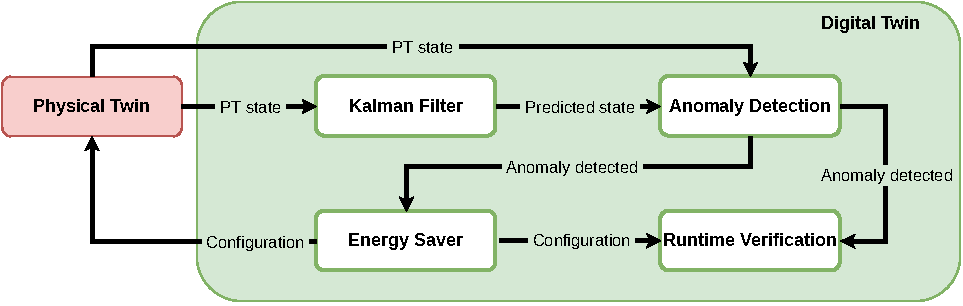
\includegraphics[width=\columnwidth]{images/incubator_anomaly_HL.pdf}
	\caption{High-level overview of the DT components relevant to the examples below. Arrows indicate RabbitMQ messages and associated data.}
	\label{fig:incubator}
\end{figure}
